\chapter{Oracle Aplication Express}


\section{Tahapan Pembuatan Aplikasi Oracle Apex}
Langkah pertama yang harus dilakukan masuk ke aplikasi Apex yang sudah didaftar pada praktikum sebelumnya, setelah semuanya berhasil langsung saja ketahap Aplication builder:
\begin{enumerate}
\item[1]Bertikut Tampilan Aplication Builder

\begin{figure}[!htbp]

    \begin{center}
        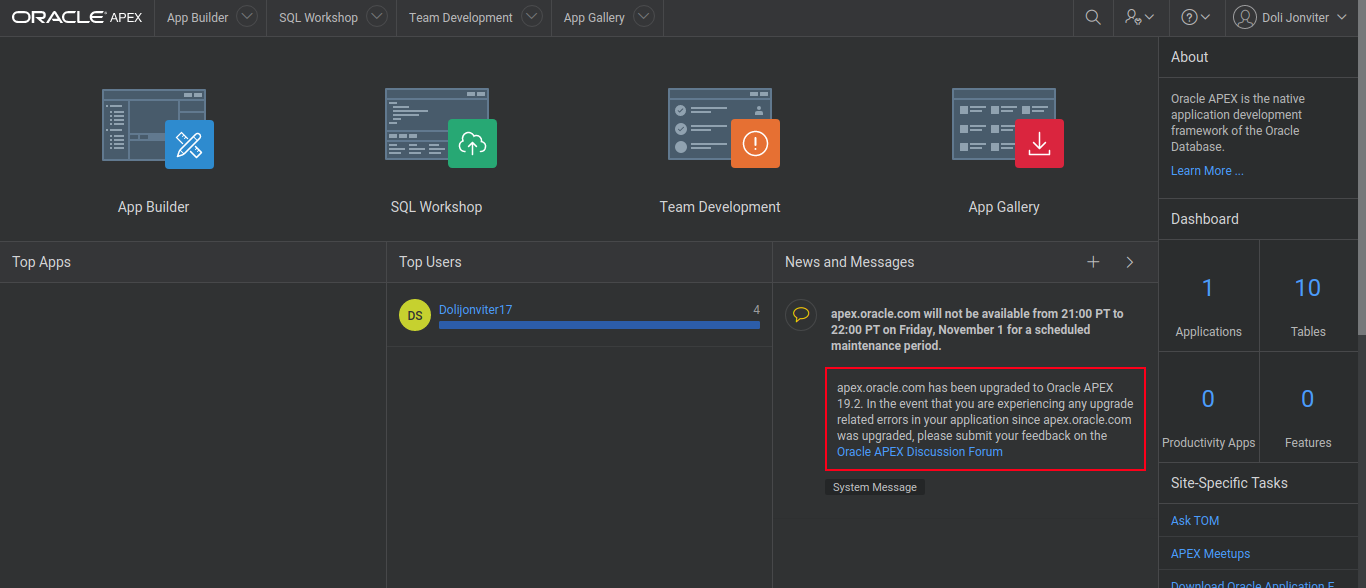
\includegraphics[scale=0.3]{figures/halamanApex.png}
        \caption{\textit{Tampilan Utama Apex}}
        \end{center}   
        \end{figure}
        \begin{figure}[!htbp]


\item[2] Buka App Builder lalu klik Create New App.

    \begin{center}
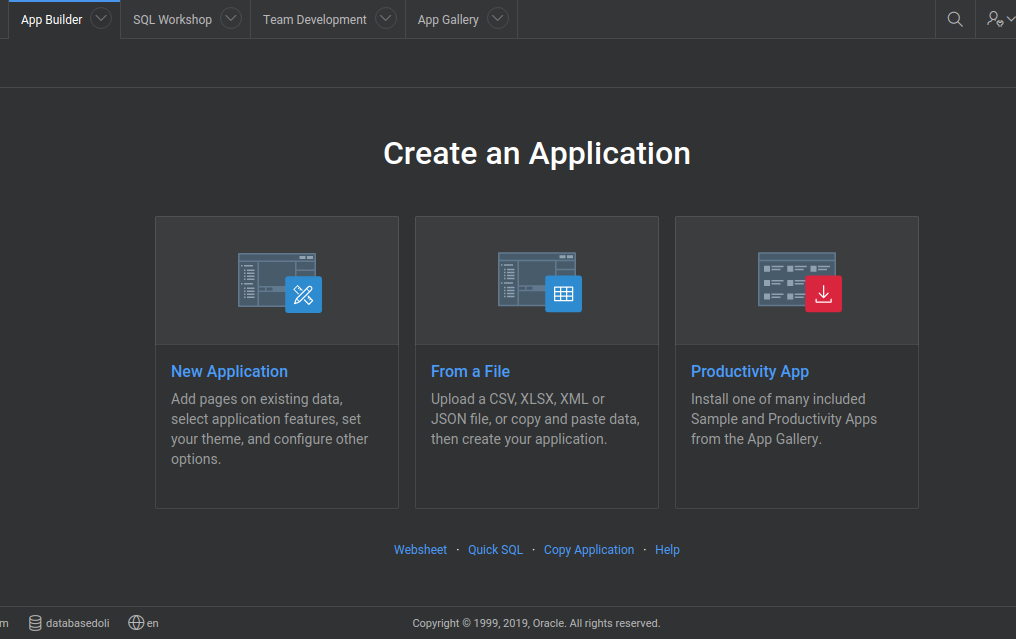
\includegraphics[scale=0.4]{figures/createAppFromfile.png}
    \caption{\textit{Oracle Apex App Builder}}
        \end{center}
\label{gambar}
\end{figure}

\begin{figure}

\item[3] Memilih Sampel Data untuk digunakan

    \begin{center}
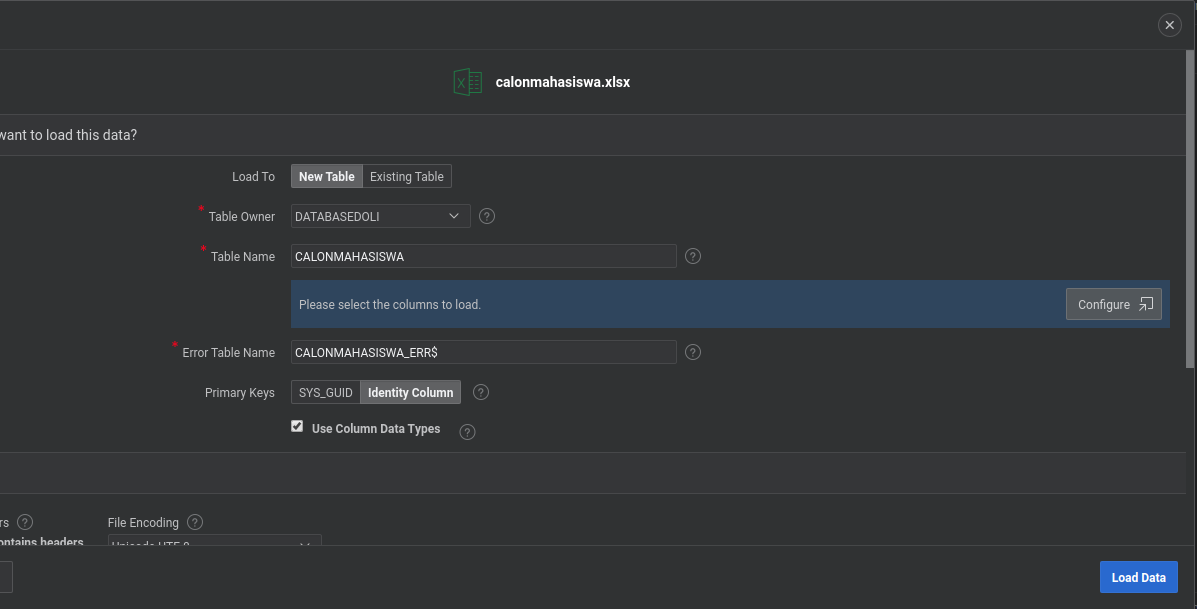
\includegraphics[scale=0.3]{figures/dataexel.png}
    \caption{\textit{Load Data.}}
        \end{center}
\label{gambar}
\end{figure}


\begin{figure}
\item[4] Sukses Import data exel.

    \begin{center}
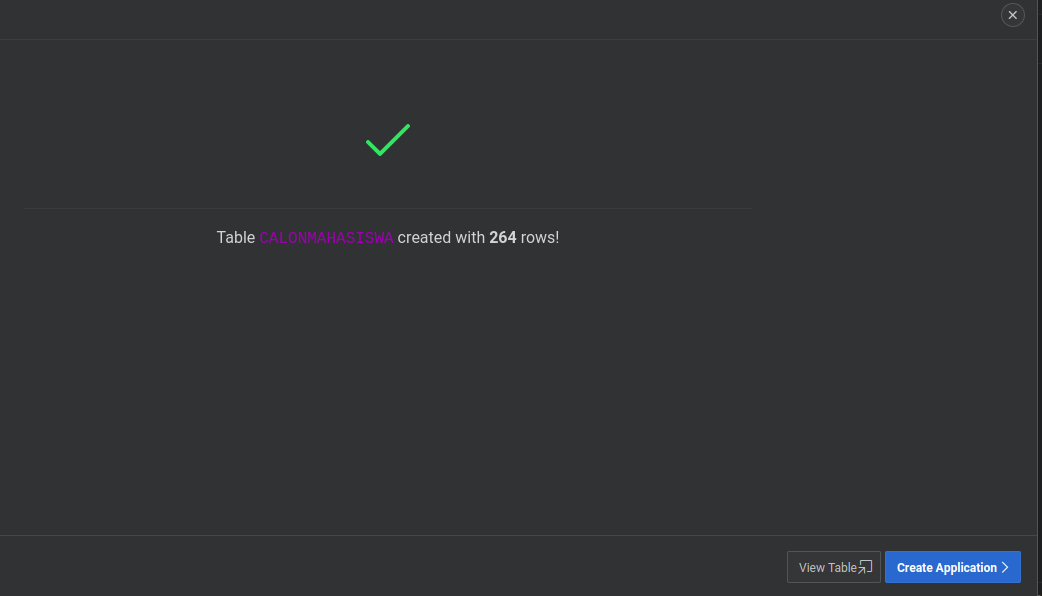
\includegraphics[scale=0.2]{figures/sukses.png}
    \caption{\textit{Import Data Sukses.}}
        \end{center}
\label{gambar}
\end{figure}


\begin{figure}
\item[5]Create Application .

    \begin{center}
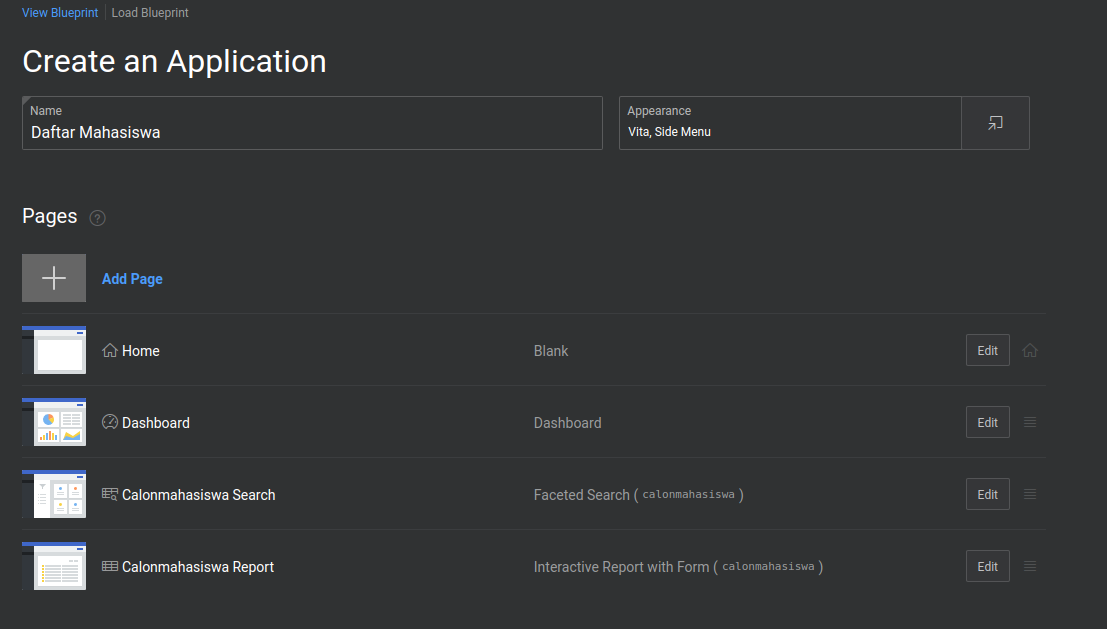
\includegraphics[scale=0.4]{figures/daftarmhs.png}
    \caption{\textit{Create an Application}}
        \end{center}
\label{gambar}
\end{figure}

\begin{figure}

\item[6]Setelah selesai mengimport file dan membuat nama tabel maka aplikasi akan melakukan running untuk menuju halaman login .

    \begin{center}
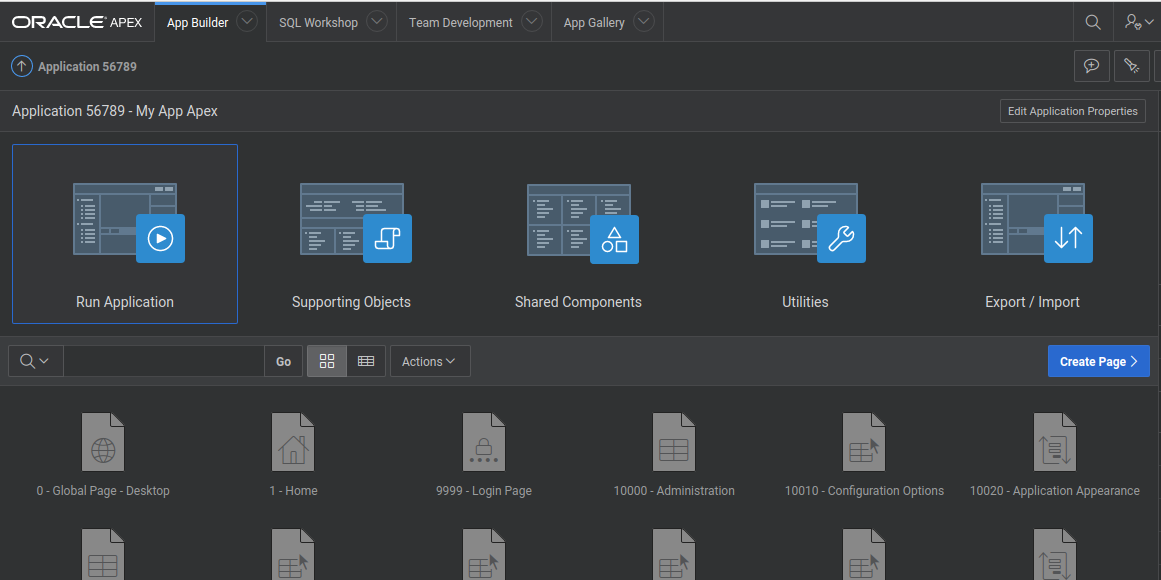
\includegraphics[scale=0.4]{figures/tampilaApp.png}
    \caption{\textit{App Builder Success}}
        \end{center}
\label{gambar}
\end{figure}

\begin{figure}
\item[7]Login untuk melihat aplikasi yang sudah dibuat sebelumnya.

    \begin{center}
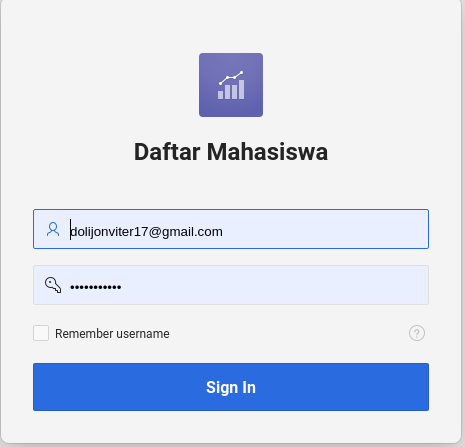
\includegraphics[scale=0.4]{figures/loginMhs.png}
    \caption{\textit{Sign In Spreadsheet}}
        \end{center}
\label{gambar}
\end{figure}

\begin{figure}
\item[8]Hasil Akhir.

    \begin{center}
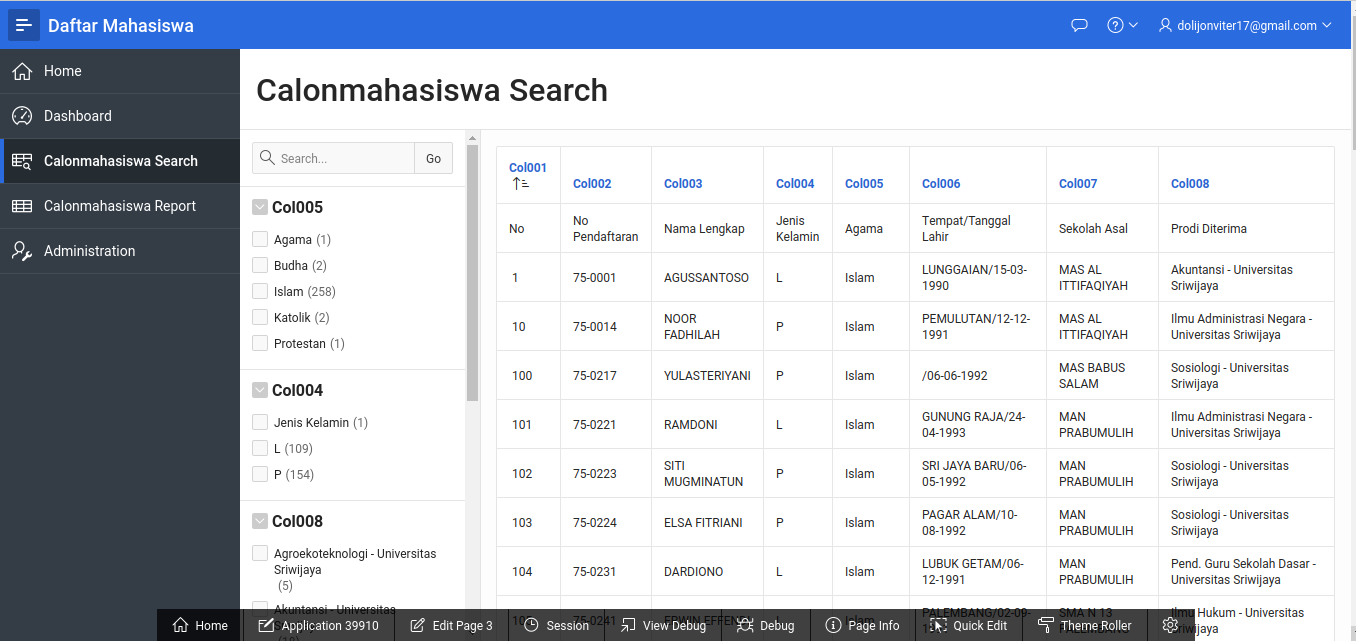
\includegraphics[scale=0.3]{figures/mhs1.png}
    \caption{\textit{Welcome Spreadsheet}}
        \end{center}
\label{gambar}
\end{figure}

\end{enumerate}




    

